%%%%%%%%%%%%%%%%%%%%%%%%%%%%%%%%%%%%%%%%%%%%%%%%%%%%%%%%%%%%%%%%%%%%%%%%%%%%%%%
% ICML 2025 SUBMISSION DRAFT: Event-based Tactile Pole Balancing
%%%%%%%%%%%%%%%%%%%%%%%%%%%%%%%%%%%%%%%%%%%%%%%%%%%%%%%%%%%%%%%%%%%%%%%%%%%%%%%

\documentclass{article}

% Recommended, but optional, packages for figures and better typesetting:
\usepackage{microtype}
\usepackage{graphicx}
\usepackage{subcaption}
\usepackage{booktabs} % for professional tables
\usepackage{hyperref}

% Attempt to make hyperref and algorithmic work together better:
\newcommand{\theHalgorithm}{\arabic{algorithm}}

% Use the following line for the initial blind version submitted for review:
% \usepackage{icml2025}
% If accepted, instead use the following line for the camera-ready submission:
\usepackage[accepted]{icml2025} % using [accepted] to show author names in draft

% For theorems and such
\usepackage{amsmath}
\usepackage{amssymb}
\usepackage{mathtools}
\usepackage{amsthm}

% if you use cleveref..
\usepackage[capitalize,noabbrev]{cleveref}

\icmltitlerunning{Learning Pole Balancing via Event-based Tactile Early Fusion}

\begin{document}

\twocolumn[
\icmltitle{Learning Pole Balancing via Event-based Tactile Early Fusion: \\
           A Comparative Analysis of Angular and Vectorial Representations}

\icmlsetsymbol{equal}{*}

\begin{icmlauthorlist}
\icmlauthor{Victor P. S. Pepe}{equal,tud,usp}
\icmlauthor{Thiago Daquino Velasquez}{equal,tud,usp}
\icmlauthor{Bárbara Fernandes Dias Bueno}{equal,tud,usp}
\icmlauthor{Tim Schneider}{tud}
\icmlauthor{Niklas Fund}{tud}
\end{icmlauthorlist}

\icmlaffiliation{tud}{Department of Electrical Engineering and Information Technology, TU Darmstadt, Darmstadt, Germany}
\icmlaffiliation{usp}{Polytechnic School, University of São Paulo (Poli-USP), São Paulo, Brazil}

\icmlcorrespondingauthor{Victor P. S. Pepe}{victor.pepe@stud.tu-darmstadt.de}
\icmlcorrespondingauthor{Thiago Daquino Velasquez}{thiago.velasquez@stud.tu-darmstadt.de}

\icmlkeywords{Machine Learning, ICML, Tactile Sensing, Event-based Vision, Robotics, Deep Learning, Pole Balancing}

\vskip 0.3in
]

\printAffiliationsAndNotice{\icmlEqualContribution} 

\begin{abstract}
    Precise estimation of object orientation from tactile feedback is critical for robotic manipulation, particularly in scenarios where visual sensing is unreliable or unavailable. We study 3D pole orientation estimation from high-resolution tactile time-series data, motivated by tactile-based pole balancing, and formulate the problem as regression on the unit sphere $S^2$. Direct learning from raw tactile pressure maps is challenged by high dimensionality and spatial redundancy, which we address through a Statistical Multi-Quad encoding that aggregates activations into structured spatial-statistical features at multiple resolutions. Ground-truth orientation vectors are computed from optical marker data via Singular Value Decomposition (SVD), and evaluation employs strict temporal splits across recording sessions to prevent interpolation-induced leakage. We compare memoryless, short-term temporal, and long-horizon sequence models under multiple target parameterizations. Our results show that \textbf{[BEST MODEL CONFIGURATION]} achieves the lowest mean angular error of \textbf{[X.X$^\circ$]} on temporally separated recording sessions, highlighting the importance of structured tactile representations combined with temporal modeling for accurate and stable orientation regression.
    \end{abstract}

\section{Introduction}
\label{intro}

Pole balancing is a classic benchmark in control theory and robotics, requiring precise and low-latency feedback to maintain an inherently unstable system. Traditional vision-based systems often suffer from motion blur and high latency, limiting their effectiveness in highly dynamic manipulation tasks. In this work, we leverage neuromorphic tactile sensing, which provides asynchronous, event-based data with microsecond resolution.

Our primary contribution is twofold: (i) an efficient statistical strategy for event-feature extraction using multi-quadrant spatial pooling, and (ii) an empirical evaluation of different output head geometries for orientation estimation, providing a generalized framework for evaluating regression models in 3D space.

\section{Background}
-evtac sensor, (not us)
\section{Related Work}
- evtac e como ele coleta dados
- trabalhos q tentam estimar angulo do pole de diversas formas.
- tactile pose estimation
\section{Methodology}
\subsection{Problem Formulation}
- o objetivo final é equilibrar o pole.
- temos as informações de estado do robo, e os eventos do sensor tátil.
- queremos prever a orientação do POLE.
- com isso, podemos usar controladores clássicos para manter o equilíbrio.
\subsection{Data Collection}
We opted to collect real human data to train the proposed model in order to capture realistic interaction dynamics,
sensor noise, and natural variability, that would not be able to be fully replicated in a simulated environment.
The human data collection also proved to be better for capturing more extreme pole angles, differently from a robotic setup where the pole would likely fall after reaching such angles.

For that pourpose, we designed a custom handle equipped with an \textit{Evtac} tactile sensor, and a set of \textit{OptiTrack} markers.
This handle was used by human operators, to perform the balancing task, while the tactile and motion capture data were recorded simultaneously.

Ground-truth measurements of the pole angle together with handle angle and position were obtained using an \textit{OptiTrack} motion capture system, which provides accurate 3D pose estimation.
The motion capture data was temporally synchronized with the tactile sensor readings to ensure alignment between input signals and target labels.

Aiming to obtain a more varied dataset, we recorded multiple sessions with two different team members.
Also, to ensure a fair and unbiased evaluation, one complete recording from each member were reserved exclusively for testing.
This recordings were not used during training or validation. The remaining data was split into training and validation sets.
All evaluated models were trained and validated using exactly the same data to guarantee a consistent comparison.

\begin{figure}[htbp]
    \centering
    
    \begin{subfigure}{0.48\linewidth}
        \centering
        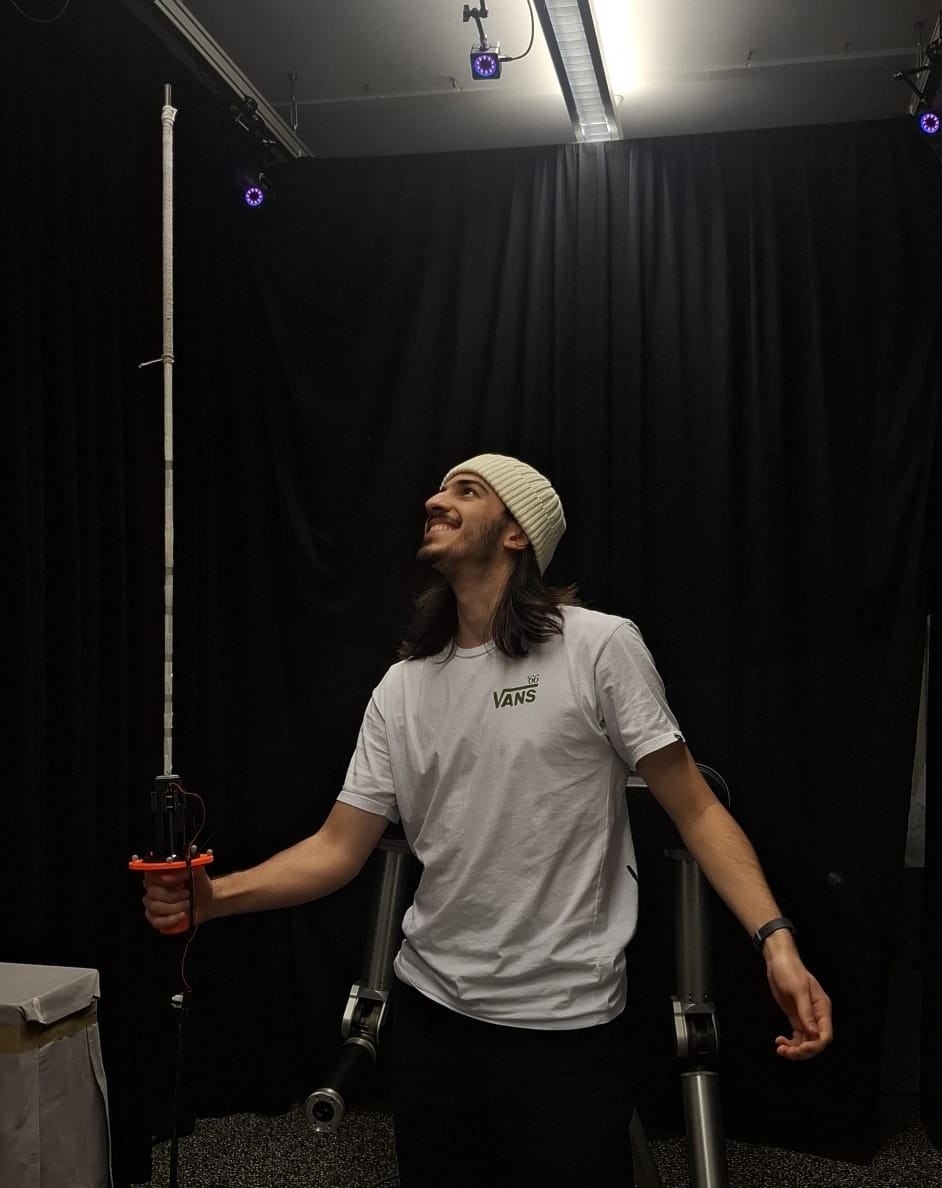
\includegraphics[width=\linewidth]{images/thiago_balancing.jpeg}
        \caption{One of the team members performing the pole balancing task.}
        \label{fig:img1}
    \end{subfigure}
    \hfill
    \begin{subfigure}{0.48\linewidth}
        \centering
        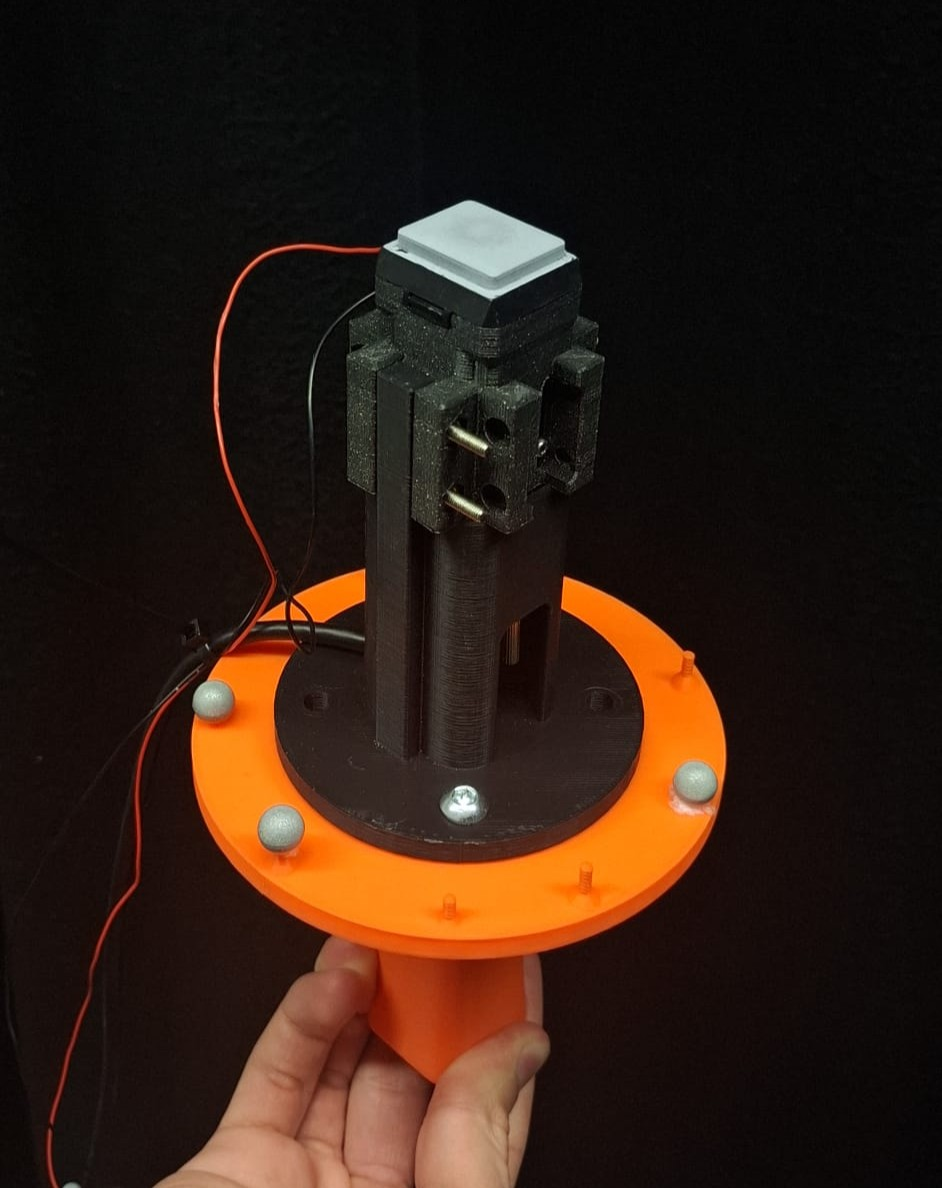
\includegraphics[width=\linewidth]{images/holder.jpeg}
        \caption{Personalized handle equipped with an \textit{Evtac} tactile sensor and \textit{OptiTrack} markers.}
        \label{fig:img2}
    \end{subfigure}
    
    \caption{Human data collection setup.}
    \label{fig:comparison}
\end{figure}

\subsection{Metrics}
\subsubsection{Loss Functions}
For the angular representation, standard Mean Squared Error (MSE) is applied. For the vectorial representation, we employ the Cosine Embedding Loss, defined as:
\begin{equation}
\mathcal{L}(\mathbf{v}, \hat{\mathbf{v}}) = 1 - \cos(\mathbf{v}, \hat{\mathbf{v}})
\end{equation}
By setting the target similarity to $1$, this loss directly optimizes the alignment between the predicted and ground truth orientation vectors. 

\subsubsection{Universal Metric: Mean Angular Error}
Comparing an angular model against a vectorial model requires an agnostic evaluation metric. We introduce a decoupled post-processing function that maps any model output back to a 3D unit vector. Performance is universally tracked using the \textit{Mean Angular Error} ($\text{MAE}_{\text{deg}}$):
\begin{equation}
\text{MAE}_{\text{deg}} = \frac{180}{\pi} \frac{1}{M} \sum_{i=1}^M \arccos \left( \operatorname{clamp}(\hat{\mathbf{v}}_i \cdot \mathbf{v}_i, -1, 1) \right)
\end{equation}
where $M$ is the batch size. This formulation provides a physically interpretable measure of the network's spatial deviation.

\subsubsection{Output Representations}
We contrast two strategies for predicting the pole orientation $\mathbf{y}$:
\begin{enumerate}
    \item \textbf{Vectorial Head:} Predicts a 3D vector $\hat{\mathbf{v}} \in \mathbb{R}^3$, followed by an $L_2$ normalization layer to guarantee a unit direction vector $||\hat{\mathbf{v}}|| = 1$.
    \item \textbf{Angular Head:} Predicts Euler angles $(\hat{\phi}, \hat{\theta})$, representing azimuth and elevation.
\end{enumerate}

\subsection{Arquitectures}
- explicar todas as arquiteturas e modelos usados.
\subsection{Framework}
- explicar o frameork que criamos, e a importãncia dele
- The models were trained using the AdamW optimizer with a Reduce-LROnPlateau scheduler. Hyperparameter tuning and model tracking were managed via Hydra and MLflow, ensuring strict decoupling between the model definition and the training loop. 
\section{Experiments}
- explicar as combinações feitas dos modelos, valores utilizados e porque.
\section{Results}
- resultados de cada experimento
- discussão em cima disso
\section{Conclusion and feature work}
Our findings suggest that vectorial representation is significantly more robust for high-frequency tactile feedback in pole balancing tasks. The event-based statistical pooling strategy successfully balances low latency with sufficient spatial acuity. Future work will explore the integration of Recurrent Neural Networks (RNNs) and Spiking Neural Networks (SNNs) to capture the temporal dynamics of the event stream natively.


\bibliography{example_paper}
\bibliographystyle{icml2025}

\end{document}
